\documentclass{sig-alternate-ipsn13}

\begin{document}

\title{BPM: Bluetooth Parking Manager}

\numberofauthors{2}

\author{
% 1st. author
\alignauthor
Wookjong Kwak\\
       \affaddr{Carnegie Mellon University Silicon Valley}\\
       \affaddr{Moffett Field}\\
       \affaddr{California 94035}\\
       \email{wookjong.kwak@sv.cmu.edu}
% 2nd. author
\alignauthor
Sungho Cho\\
       \affaddr{Carnegie Mellon University Silicon Valley}\\
       \affaddr{Moffett Field}\\
       \affaddr{California 94035}\\
       \email{sungho.cho@sv.cmu.edu}
}

\maketitle
\begin{abstract}

The goal of our parking lot gate opening system is providing seamless authentication without additional user effort and additional device. We propose to use Bluetooth technology as a communication channel with smartphone as a control device. Given that most smartphones have embedded Bluetooth module, and most users bring their device in everyday life, especially when driving, the combination of Bluetooth with smartphone is a strong candidate for our solution. We will also use different sensors to verify location of the user to eliminate possibilities of granting access to unauthorized users.

\end{abstract}

\keywords{Android, Arduino, Bluetooth}

\section{Introduction}

According to \cite{national}, the United States parking industry is an \$18 billion dollar industry, and there are more than 40,000 parking facilities in the United States. \cite{ibisworld} also reported that the revenue of the parking lots and garages industry has reached \$9 billion dollars, and over 136,000 employments and 8,000 businesses are involved with the industry. Although the industry has been decreasing for the past five years mostly due to the recession and under capacity of airport parking lots, \cite{ibisworld} had reported that the demand will pick up in the next five years as employment improves and demand from airports and other businesses revives. 

The access of these parking lots and garages are managed through different types of gate openers, and they are mostly operated with access card using RFID or dispensing paper tickets to customers. Although the gated parking lots and garages provide more security and guaranteed parking spaces, there are few problems to both users and the parking service providers in current systems. The most cumbersome task users have to bear with is physically swiping the access card to the reader or inserting the paper ticket to the machine to open the gate. As the result, it creates extra user actions such as finding the access card or the paper ticket, opening the window, and finally swiping the access card or inserting the paper ticket to the machine. From the service provider's perspective, it is inconvenient to issue a new access card or a paper ticket for each new client. For the access card, it is hard to retrieve or revoke expired access cards.

Through our BPM (Bluetooth Parking Manager) system, we demonstrate that users can easily use parking lots and garages with minimum user action using Bluetooth technology embedded in their smartphones. In our approach, we allow users to easily purchase parking permits through our client Android application, and seemlessly control the gates of desired parking lots and garages using Bluetooth communication channel between the user's smartphone and the Bluetooth module which controls the gate. Additionally, our approach only requires attaching a Bluetooth module to the current parking lot system, which is a low cost solution. It allows most parking lot service providers to implement the solution and improve their parking lot and garage services.
\section{Related Work}

There has been active and extensive researches focusing on improving the parking lot and garage user experience. Motorola has been actively researching Automatic License Plate Recognition system \cite{alpr}, which reads the vehicle's license plates and checks them against the database to quickly identify the verification of vehicles (as shown in Figure \ref{fig:alpr}). This system has been widely used not only the parking ticketing systems, but also locating stolen or wanted vehicles, tolling, boarder control, etc. As the name of the system indicates, this system uses illumination, such as infra-red, and a camera to take the image of the license plate of vehicles, then analyzes the image with an image-processing software to extract the license plate information. Once the license plate information has been extracted, it is checked against the database to identify the vehicle, and the parking lot gates opens automatically if the vehicle is authorized to use the parking lot \cite{lpr}. This system has an advantage of not requiring any installation on the vehicle.

\begin{figure}[ht]
	\centering
		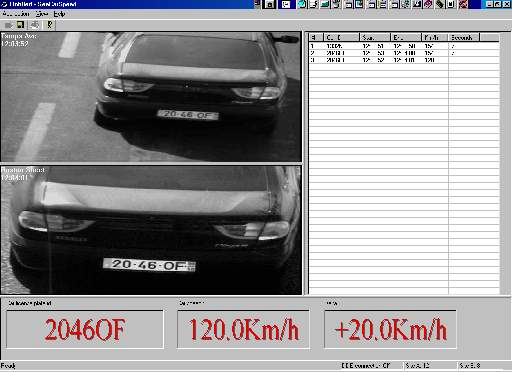
\includegraphics[width=3in]{figure/alpr.jpg}
		\caption{Automatic License Plate Recognition system takes an image of the vehicle and extracts the license plate information}
	\label{fig:alpr}
\end{figure}

However, such system requires a major upgrade in the parking lot, because it requires a completely different set of components, such as cameras, illumination, frame grabber, computer, and image-processing software. 	These equipments can be very expensive, in order to achieve a certain level of accuracy. This high cost of the system is not very appealing to the parking lot service providers. Additionally, the external effects, such as sun and headlights, and bad license plates, can severely affect the performance of the system. 

The rest of this paper will explain the system overview of our low-cost parking lot system, followed by the details of the system, evaluation, and conclusion.
\section{System Overview}

The BPM system can be broadly divided into three components (as shown in Figure \ref{fig:sys_overview}). The first component is the client Android application. It is the core component of the BPM system, which provides an interface allowing users to register with our system. In addition, the application also allows users to easily look up available parking lots and buy permits for desired parking lots. Another main task of the Android application is scanning available Bluetooth devices around the user. It periodically scans a discoverable Bluetooth device which is attached to the gate of parking lot or garage. 

\begin{figure}[ht]
	\centering
		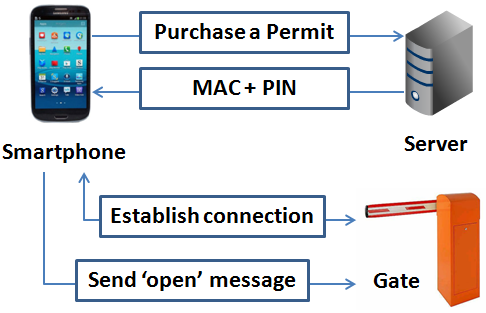
\includegraphics[width=3in]{figure/sys_overview.png}
		\caption{The BPM system consists of three components: client Android application, server, and Bluetooth enabled parking lot gate}
	\label{fig:sys_overview}
\end{figure}

The second component is the application server, which provides RESTful end-points for useful functions that are used by the client Android application. These functions include registration, parking lot searching, buying parking lot permits, etc. When a user registers with our system, he/she may search for parking lots simply buy providing a ZIP code, which then the server retrieves available parking lots and garages for the user. Oncec the user purchases the permit, the server returns the MAC address of the particular parking lot's Bluetooth device and the PIN associated with the Bluetooth device for pairing to establish a communication channel between the user's smartphone and the Bluetooth device.

The last component is the Bluetooth device which is attached to the gate of parking lot. It is essentially a combination of an Arduino board and a Bluetooth module. Once the user purchases the permit, the user's smartphone maintains the MAC address and the PIN. Once the client Android application finds the correct Bluetooth device by matching with the MAC address, it automatically initiates pairing process and establishes a communication channel. Once the communication channel is successfully established, the client Android application sends a message to the parking lot Bluetooth device to open the gate. The parking lot Bluetooth receives the message and command the gate to open via the Arduino board attached to the gate.
\section{System Details}

\section{Evaluation}
\subsection{Signal Strength Threshold}
Once we build a basic service flow, we needed to set up the threshold of Bluetooth signal strength to determine when the system will open up the gate depending on how far the user is. Since we presumed that the distance to user from the parking lot gate attached to Bluetooth module is correspond the signal strength, we needed empirical data to evaluate the system efficiency and stability.

Thus, we performed experiments to collect signal strength of Bluetooth with the android device after setting up a practical environment outside. We put the two cars in a row and collected signal strength inside of each car, first car in front and second car behind.

Figure~\ref{fig:comparison} shows the comparison between the collected data for 60 seconds in the first car and the second car. As a result of plentiful of experiments, 10 minutes * 3 times in a day * 3 days, we observed that the range of signal strength in the first car was -67 to -83 and -86 to -96 (or less). Bold line represents the median value of collected data.

\begin{figure}
	\centering
	\begin{subfigure}[b]{.5\linewidth}
		\centering
		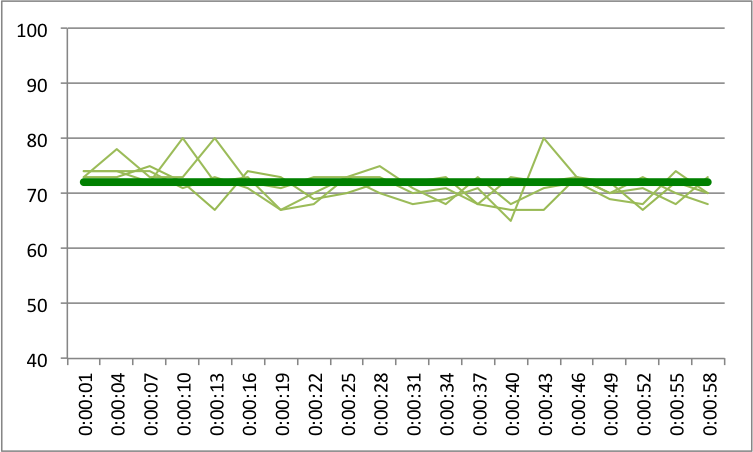
\includegraphics[width=1.5in]{figure/bt_first_car}
		\caption{The first car in front}
		\label{fig:first car}
	\end{subfigure}%
	\begin{subfigure}[b]{.5\linewidth}
		\centering
		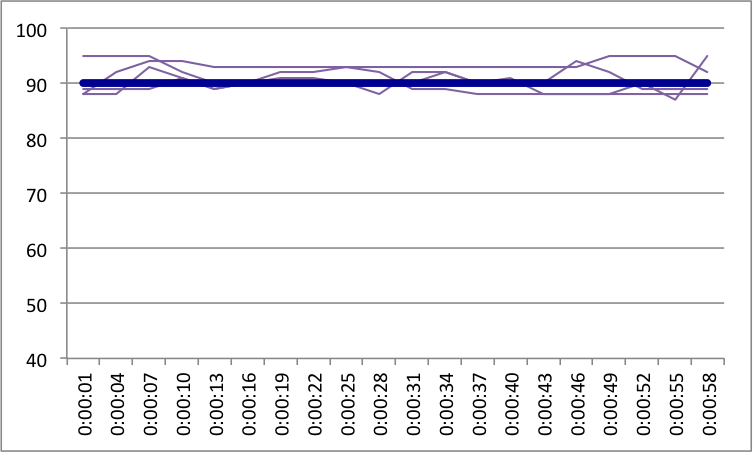
\includegraphics[width=1.5in]{figure/bt_second_car}
		\caption{The second car behind}
		\label{fig:second car}
	\end{subfigure}
	\caption{RSSI Comparison between two cars}
	\label{fig:comparison}
\end{figure}

Based on the analysis, we set the threshold at -85 and it returned desirable result to an extend that it prevents perfectly for even a corner case problem that unregistered user in front gets in to the gate piggybacking the grant of user behind. What it means is the system only opens the gate for the user who is within a range of about a car length.
\subsection{Discovery Latency}
In addition, to evaluate the performance of our system regarding latency, we also measured waiting time to open the gate, while the vehicle is in motion and in stillness. Through this experiment, we observed that the waiting time is truly random whether the vehicle is moving or not. This is because the Bluetooth discovery process in Android usually takes 12 seconds of inquiry scan cycle \cite {btcycle}. In order words, at any moment during 12 seconds, the Bluetooth module can be found and the user might have no waiting time to 12 seconds of waiting time, at most.

This limitation made us cannot use average value of multiple samples to set up the threshold. Since, suppose, we want to collect 5 samples for averaging out, then the user has to wait 60 seconds in worst-case scenario.

\section{Conclusion}

%\begin{figure}
%\centering
%\epsfig{file=fly.eps}
%\caption{A sample black and white graphic (.eps format).}
%\label{fig:example}
%\end{figure}

%
% The following two commands are all you need in the
% initial runs of your .tex file to
% produce the bibliography for the citations in your paper.
\bibliographystyle{abbrv}
\bibliography{sigproc}  % sigproc.bib is the name of the Bibliography in this case
% You must have a proper ".bib" file
%  and remember to run:
% latex bibtex latex latex
% to resolve all references
%
% ACM needs 'a single self-contained file'!
%
%APPENDICES are optional
%\balancecolumns
%\appendix
%Appendix A

%Appendix goes here.

% That's all folks!
\end{document}
